\documentclass[10pt]{article}

\usepackage[T1]{fontenc}
\usepackage[utf8]{inputenc}
%\usepackage{beton}
%\usepackage{ccfonts}
%\usepackage{concrete}
\usepackage{concmath}
\usepackage{eulervm}
\usepackage{amsmath,amsthm,amssymb}
\usepackage{mathtools}
\usepackage{multicol}
\usepackage{marginnote}
\usepackage{pgfplots}
\usepackage{float}
\usepackage{hyperref}
\usepackage{bbm}
\usepackage{booktabs}
\pgfplotsset{compat=1.5}

\usepackage{listings}
\usepackage{xcolor}
\definecolor{codegreen}{rgb}{0,0.6,0}
\definecolor{codegray}{rgb}{0.5,0.5,0.5}
\definecolor{codepurple}{rgb}{0.58,0,0.82}
\definecolor{backcolour}{rgb}{0.95,0.95,0.92}
\lstdefinestyle{mystyle}{
    backgroundcolor=\color{backcolour},   
    commentstyle=\color{codegreen},
    keywordstyle=\color{magenta},
    numberstyle=\tiny\color{codegray},
    stringstyle=\color{codepurple},
    basicstyle=\ttfamily\footnotesize,
    breakatwhitespace=false,         
    breaklines=true,                 
    captionpos=b,                    
    keepspaces=true,                 
    numbers=left,                    
    numbersep=5pt,                  
    showspaces=false,                
    showstringspaces=false,
    showtabs=false,                  
    tabsize=2
}

\lstset{language=Python, style=mystyle}

\usepackage{mathtools}

\usepackage{wasysym}
\usepackage[margin=1.5in]{geometry} 
\usepackage{enumerate}
\index{\usepackage}\usepackage{multicol}

\newcommand{\N}{\mathbf{N}}
\newcommand{\Z}{\mathbb{Z}}

\newcommand{\R}{\mathbf{R}}
\newcommand{\C}{\mathbf{C}}
\newcommand{\Pbb}{\mathbb{P}}
\newcommand{\Fcal}{\mathcal{F}}
\newcommand{\Lcal}{\mathcal{L}}
\newcommand{\Acal}{\mathcal{A}}
\newcommand{\Ecal}{\mathcal{E}}
\newcommand{\Ebb}{\mathbb{E}}
\newcommand{\Qbb}{\mathbb{Q}}


\renewcommand{\mathbf}{\mathbold}

\newenvironment{theorem}[2][Theorem]{\begin{trivlist}
  \item[\hskip \labelsep {\bfseries #1}\hskip \labelsep {\bfseries #2.}]}{\end{trivlist}}
\newenvironment{lemma}[2][Lemma]{\begin{trivlist}
  \item[\hskip \labelsep {\bfseries #1}\hskip \labelsep {\bfseries #2.}]}{\end{trivlist}}
\newenvironment{exercise}[2][Exercise]{\begin{trivlist}
  \item[\hskip \labelsep {\bfseries #1}\hskip \labelsep {\bfseries #2.}]}{\end{trivlist}}
\newenvironment{reflection}[2][Reflection]{\begin{trivlist}
  \item[\hskip \labelsep {\bfseries #1}\hskip \labelsep {\bfseries #2.}]}{\end{trivlist}}
\newenvironment{proposition}[2][Proposition]{\begin{trivlist}
  \item[\hskip \labelsep {\bfseries #1}\hskip \labelsep {\bfseries #2.}]}{\end{trivlist}}
\newenvironment{corollary}[2][Corollary]{\begin{trivlist}
  \item[\hskip \labelsep {\bfseries #1}\hskip \labelsep {\bfseries #2.}]}{\end{trivlist}}

\newenvironment{definition}[2][Definition]{\begin{trivlist}
  \item[\hskip \labelsep {\bfseries #1}\hskip \labelsep {\bfseries #2.}]}{\end{trivlist}}

\begin{document}
	
  \renewcommand{\qedsymbol}{\smiley}
	\title{Investments Class \\ Problem set 4}
	\author{Daniel Grosu, William Martin, Denis Steffen}
	
	\maketitle

  \begin{exercise}{1}
   
\end{exercise}

\newpage

\begin{exercise}{2}

	After downloading the daily returns on the Amazon stock from CRSP, the CRSP value-weighted market return, and the short-term t-bill from 2009 to 2019, we plot our results
	
	\begin{figure}[H]
	
		\centering
		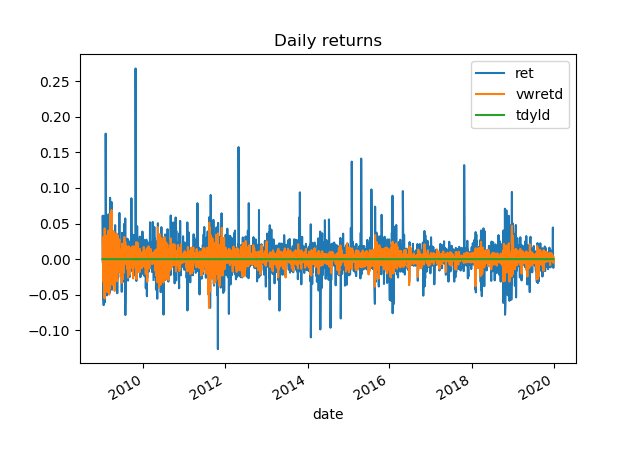
\includegraphics[scale=0.8]{figures/ex2_1.png}	
		\caption{Daily returns for 10 years of the Amazon stock (ret), the CRSP value-weighted  market return (vwretd) and the short-term t-bill (tdyld)}	
		\label{fig:ex2_1}	
	
	\end{figure} 
	
 	Before continuing our analysis, we compute the excess returns using the t-bill rate as the risk-free rate. We then compute the covariance matrix of these excess returns which gives us
	
	\begin{align*}
		\begin{pmatrix}
			0.000447 & 0.000117\\
			0.000117 & 0.000107
		\end{pmatrix}			
	\end{align*}	 
	
	Where the first element of the diagonal represents the variance of the excess returns on the Amazon stock and the second element of the diagonal the variance of the excess returns on the CRSP value-weighted market return. The non-diagonal elements are simply the covariance elements of the 2 aforementioned quantities. 	
	
	\smallbreak
	
	Computing the beta becomes straightforwards
	
	\begin{align*}
		\beta = \frac{Cov(R, R_{M})}{Var(R_{M})} = 1.091364
	\end{align*}

	We now plot the rolling-window estimate of the beta of the stock using six month data-window. We also plot the adjusted beta series using the Bloomberg formula 
	
	\begin{align*}
		\beta_{adj} = w \times \beta_{est} + (1 - w) \times \beta_{avg}
	\end{align*}
	
	Where $\beta_{avg} = 1 $ and $w = 2/3$. We also plot the constant beta found above.
	
	\begin{figure}[H]
	
		\centering
		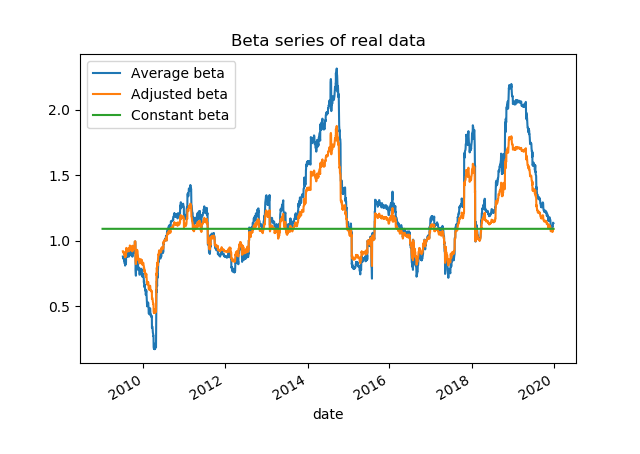
\includegraphics[scale=0.8]{figures/ex2_2.png}	
		\caption{Beta series of rolling-window estimate of beta, adjusted beta and constant beta using real data}	
		\label{fig:ex2_2}
				
	\end{figure}	

	We now simulated 10 years of data of excess returns for a stock that satisfies the CAPM equation. Using the formula below, we are able to compute idiosyncratic risk of the stock
	
	\begin{align*}
		Var(\epsilon) = Var(R) - \beta^{2} Var(R_{M})
	\end{align*}
	
	Below is the plot of the rolling-window estimate for the beta using simulated data this time (together with the adjusted and constant beta series)
	
	\begin{figure}[H]
	
		\centering
		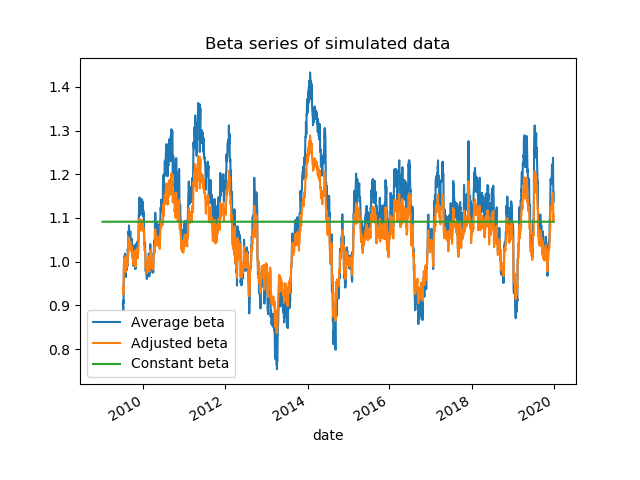
\includegraphics[scale=0.8]{figures/ex2_3.png}	
		\caption{Beta series of rolling-window estimate of beta, adjusted beta and constant beta using simulated data}	
		\label{fig:ex2_2}
				
	\end{figure}
		
\end{exercise}
  
\end{document}
